\PassOptionsToPackage{table}{xcolor}
\documentclass[aspectratio=169,10pt]{beamer}

\usepackage{lmodern}

% ── Strip all default Beamer decoration ───────────────────────────────────────
\setbeamertemplate{navigation symbols}{}
\setbeamertemplate{headline}{}

% ── Light palette ─────────────────────────────────────────────────────────────
\definecolor{primary}{HTML}{1A5276}    % dark navy-blue
\definecolor{primarylt}{HTML}{D6EAF8}  % very light blue
\definecolor{teal}{HTML}{148F77}       % teal for accents
\definecolor{teallt}{HTML}{D1F2EB}     % light teal
\definecolor{accent}{HTML}{D35400}     % burnt orange
\definecolor{accentlt}{HTML}{FDEBD0}   % light orange
\definecolor{slidebg}{HTML}{FFFFFF}         % slide bg
\definecolor{panelbg}{HTML}{F2F4F4}    % light panel
\definecolor{txt}{HTML}{1C2833}        % near-black text
\definecolor{txtsub}{HTML}{626567}     % muted text
\definecolor{pgreen}{HTML}{1E8449}     % positive green
\definecolor{pgreenlt}{HTML}{D5F5E3}   % light green
\definecolor{pred}{HTML}{C0392B}       % negative red
\definecolor{predlt}{HTML}{FADBD8}     % light red
\definecolor{codebg}{HTML}{EBF5FB}     % code background

% ── Beamer base colors ────────────────────────────────────────────────────────
\setbeamercolor{normal text}{fg=txt, bg=slidebg}
\setbeamercolor{frametitle}{fg=white, bg=primary}
\setbeamercolor{structure}{fg=primary}
\setbeamercolor{itemize item}{fg=accent}
\setbeamercolor{itemize subitem}{fg=teal}
\setbeamercolor{block title}{fg=white, bg=primary}
\setbeamercolor{block body}{fg=txt, bg=primarylt}
\setbeamercolor{block title alerted}{fg=white, bg=accent}
\setbeamercolor{block body alerted}{fg=txt, bg=accentlt}
\setbeamercolor{block title example}{fg=white, bg=teal}
\setbeamercolor{block body example}{fg=txt, bg=teallt}

% ── Frame title ───────────────────────────────────────────────────────────────
\setbeamertemplate{frametitle}{%
  \begin{beamercolorbox}[wd=\paperwidth,ht=0.95cm,dp=0.20cm,
                         leftskip=0.30cm]{frametitle}%
    \vbox to 0.85cm{%
      \vfill
    \usebeamerfont{frametitle}\insertframetitle
    \ifx\insertframesubtitle\empty\else
      \hspace{0.25cm}{\color{primarylt!80}\small\itshape--- \insertframesubtitle}
    \fi
    \vfill}%
  \end{beamercolorbox}%
}
\setbeamerfont{frametitle}{size=\large,series=\bfseries}

% ── Footer ────────────────────────────────────────────────────────────────────
\setbeamertemplate{footline}{%
  \begin{beamercolorbox}[wd=\paperwidth,ht=0.35cm,dp=0.12cm]{normal text}%
    \color{txtsub}\hspace{0.4cm}\tiny IMDB Sentiment Analysis System
    \hfill
    {\color{primary}\small\insertframenumber/\inserttotalframenumber}%
    \hspace{0.4cm}
  \end{beamercolorbox}%
}

% ── Packages ──────────────────────────────────────────────────────────────────
\usepackage[utf8]{inputenc}
\usepackage[T1]{fontenc}
\usepackage{tikz}
\usepackage{listings}
\usepackage{booktabs}
\usepackage{array}
\usepackage{colortbl}
\usepackage{graphicx}
\usepackage{amsmath}
\usepackage{tcolorbox}
\tcbuselibrary{skins}
\usetikzlibrary{arrows.meta,positioning,calc,decorations.pathreplacing}

% ── Listing style ─────────────────────────────────────────────────────────────
\lstdefinestyle{py}{
  language=Python,
  backgroundcolor=\color{codebg},
  basicstyle=\ttfamily\scriptsize,
  keywordstyle=\color{primary}\bfseries,
  stringstyle=\color{pgreen},
  commentstyle=\color{txtsub}\itshape,
  numbers=left, numberstyle=\tiny\color{txtsub},
  numbersep=5pt,
  frame=none, xleftmargin=12pt,
  breaklines=true, showstringspaces=false,
  tabsize=2,
}
\lstdefinestyle{json}{
  backgroundcolor=\color{codebg},
  basicstyle=\ttfamily\scriptsize,
  stringstyle=\color{pgreen},
  frame=none, xleftmargin=6pt,
  breaklines=true, showstringspaces=false,
}

% ── tcolorbox helpers ─────────────────────────────────────────────────────────
\tcbset{
  card/.style 2 args={
    enhanced, colback=#1, colframe=#2,
    boxrule=0pt, leftrule=3pt, arc=3pt,
    top=3pt, bottom=3pt, left=6pt, right=6pt,
    fonttitle=\bfseries\scriptsize, coltitle=#2,
    title={##1},
  },
  codebox/.style={
    enhanced, colback=codebg, colframe=primary!30,
    boxrule=0pt, leftrule=3pt, arc=2pt,
    top=3pt, bottom=3pt, left=4pt, right=4pt,
  },
}

% ─────────────────────────────────────────────────────────────────────────────
\begin{document}
\setbeamercolor{background canvas}{bg=slidebg}

%% ─────────────────────────────────────────────────────────────────────────────
%% SLIDE 1 — TITLE
%% ─────────────────────────────────────────────────────────────────────────────
{
\setbeamercolor{background canvas}{bg=primary}
\begin{frame}[plain]

\begin{tikzpicture}[remember picture,overlay]
  % Subtle light circle decorations
  \fill[white,opacity=0.04]
    (current page.south east) ++(-2cm,2.5cm) circle(5.8cm);
  \fill[accent,opacity=0.12]
    (current page.north west) ++(2cm,-2cm) circle(3.2cm);
\end{tikzpicture}

\vspace{0.5cm}
\begin{columns}[c]
  %----- Left: title block
  \column{0.58\textwidth}
    {\color{primarylt}\scriptsize\texttt{Natural Language Processing \ | \ Machine Learning \ | \ REST API}}
    \vspace{0.22cm}

    {\color{white}\fontsize{26}{32}\selectfont\bfseries IMDB Sentiment}\\[3pt]
    {\color{white}\fontsize{26}{32}\selectfont\bfseries Analysis System}
    \vspace{0.22cm}

    \textcolor{accent}{\rule{6cm}{2pt}}
    \vspace{0.18cm}

    {\color{primarylt}\small
      End-to-end NLP pipeline: 7-step preprocessing,\\
      TF-IDF + Logistic Regression, deployed via\\
      FastAPI REST API with responsive web frontend.}

    \vspace{0.5cm}
    {\color{primarylt!70}\tiny
      \texttt{sentiment\_analysis\_nlp.ipynb \ | \ sentiment\_api.py \ | \ index.html}}

  %----- Right: stats panel
  \column{0.38\textwidth}
  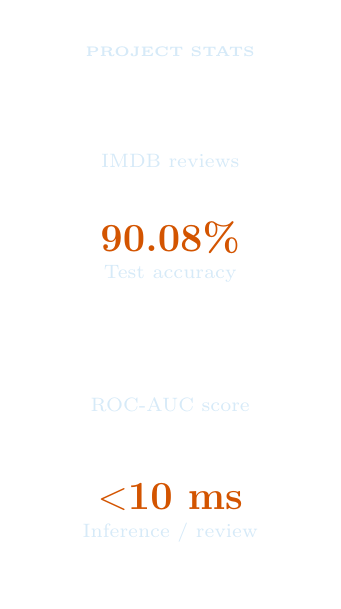
\begin{tikzpicture}
    % Panel background
    \fill[white,opacity=0.08, rounded corners=8pt]
      (-1.8,-3.6) rectangle (1.8,3.4);
    \draw[white,opacity=0.20, rounded corners=8pt, line width=0.6pt]
      (-1.8,-3.6) rectangle (1.8,3.4);

    \node[color=primarylt,font=\tiny\bfseries] at (0,3.1)
      {PROJECT STATS};

    \node[color=white,font=\Large\bfseries]   at (0, 2.2)  {50,000};
    \node[color=primarylt,font=\scriptsize]   at (0, 1.72) {IMDB reviews};

    \draw[white,opacity=0.25,line width=0.4pt] (-1.5,1.40) -- (1.5,1.40);

    \node[color=accent,font=\Large\bfseries]  at (0, 0.75) {90.08\%};
    \node[color=primarylt,font=\scriptsize]   at (0, 0.28) {Test accuracy};

    \draw[white,opacity=0.25,line width=0.4pt] (-1.5,-0.05) -- (1.5,-0.05);

    \node[color=white,font=\Large\bfseries]   at (0,-0.92) {0.9649};
    \node[color=primarylt,font=\scriptsize]   at (0,-1.38) {ROC-AUC score};

    \draw[white,opacity=0.25,line width=0.4pt] (-1.5,-1.68) -- (1.5,-1.68);

    \node[color=accent,font=\Large\bfseries]  at (0,-2.55) {$<$10 ms};
    \node[color=primarylt,font=\scriptsize]   at (0,-3.00) {Inference / review};
  \end{tikzpicture}
\end{columns}
\end{frame}
}

%% ─────────────────────────────────────────────────────────────────────────────
%% SLIDE 2 — SYSTEM OVERVIEW
%% ─────────────────────────────────────────────────────────────────────────────
\begin{frame}{System Overview}
\framesubtitle{End-to-end pipeline from raw text to deployed REST API}

\vspace{0.15cm}
% Pipeline flow
\begin{center}
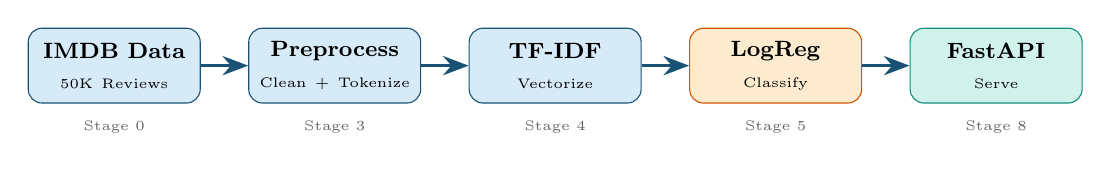
\begin{tikzpicture}[
  pnode/.style={
    draw=primary, fill=primarylt,
    rounded corners=5pt,
    minimum width=2.1cm, minimum height=0.95cm,
    align=center, text width=1.95cm, font=\small},
  hinode/.style={
    draw=accent, fill=accentlt,
    rounded corners=5pt,
    minimum width=2.1cm, minimum height=0.95cm,
    align=center, text width=1.95cm, font=\small},
  oknode/.style={
    draw=teal, fill=teallt,
    rounded corners=5pt,
    minimum width=2.1cm, minimum height=0.95cm,
    align=center, text width=1.95cm, font=\small},
  arr/.style={-{Stealth[scale=1.1]}, primary, line width=1.2pt},
]
  \node[pnode] (A) at (0,0)   {\textbf{\footnotesize IMDB Data}\\\tiny 50K Reviews};
  \node[pnode] (B) at (2.8,0) {\textbf{\footnotesize Preprocess}\\\tiny Clean + Tokenize};
  \node[pnode] (C) at (5.6,0) {\textbf{\footnotesize TF-IDF}\\\tiny Vectorize};
  \node[hinode](D) at (8.4,0) {\textbf{\footnotesize LogReg}\\\tiny Classify};
  \node[oknode](E) at (11.2,0){\textbf{\footnotesize FastAPI}\\\tiny Serve};

  \draw[arr] (A)--(B); \draw[arr] (B)--(C);
  \draw[arr] (C)--(D); \draw[arr] (D)--(E);

  \foreach \nd/\st in {A/0,B/3,C/4,D/5,E/8}{
    \node[font=\tiny,color=txtsub,below=0.1cm of \nd] {Stage \st};
  }
\end{tikzpicture}
\end{center}

\vspace{0.2cm}
\begin{columns}[T]
  \column{0.32\textwidth}
  \begin{tcolorbox}[enhanced,colback=primarylt,colframe=primary,
      boxrule=0pt,leftrule=3pt,arc=3pt,
      top=4pt,bottom=4pt,left=6pt,right=6pt,
      title={\small\bfseries\color{primary} Data Layer},
      coltitle=primary]
    \scriptsize
    \begin{itemize}\setlength\itemsep{1pt}
      \item 50,000 \texttt{.txt} IMDB reviews
      \item Balanced: 50\,\% pos / 50\,\% neg
      \item Parsed to \texttt{imdb\_reviews.csv}
      \item 80\,\% train / 20\,\% test split
    \end{itemize}
  \end{tcolorbox}

  \column{0.32\textwidth}
  \begin{tcolorbox}[enhanced,colback=accentlt,colframe=accent,
      boxrule=0pt,leftrule=3pt,arc=3pt,
      top=4pt,bottom=4pt,left=6pt,right=6pt,
      title={\small\bfseries\color{accent} ML Layer},
      coltitle=accent]
    \scriptsize
    \begin{itemize}\setlength\itemsep{1pt}
      \item 7-step NLP preprocessing
      \item TF-IDF with 10K features
      \item 5 models benchmarked
      \item LogReg wins: 90.08\,\%
    \end{itemize}
  \end{tcolorbox}

  \column{0.32\textwidth}
  \begin{tcolorbox}[enhanced,colback=teallt,colframe=teal,
      boxrule=0pt,leftrule=3pt,arc=3pt,
      top=4pt,bottom=4pt,left=6pt,right=6pt,
      title={\small\bfseries\color{teal} API Layer},
      coltitle=teal]
    \scriptsize
    \begin{itemize}\setlength\itemsep{1pt}
      \item FastAPI + Pydantic validation
      \item \texttt{/predict} and \texttt{/batch\_predict}
      \item Swagger UI auto-docs
      \item CORS + HTML5 frontend
    \end{itemize}
  \end{tcolorbox}
\end{columns}
\end{frame}

%% ─────────────────────────────────────────────────────────────────────────────
%% SLIDE 3 — DATASET
%% ─────────────────────────────────────────────────────────────────────────────
\begin{frame}{Dataset --- IMDB Movie Reviews}
\framesubtitle{50,000 balanced reviews from Stanford AI Lab (aclImdb)}

\begin{columns}[T]
  \column{0.32\textwidth}
  \vspace{0.1cm}
  {\scriptsize
  \rowcolors{2}{primarylt!60}{white}
  \begin{tabular}{@{}ll@{}}
    \toprule
    \rowcolor{primary!15}\textbf{Property} & \textbf{Value}\\
    \midrule
    Total reviews  & 50,000 \\
    Training set   & 40,000 \\
    Test set       & 10,000 \\
    Positive       & 25,000 \\
    Negative       & 25,000 \\
    Avg.\ length   & 230 words \\
    Vocabulary     & $\sim$100K \\
    TF-IDF feats   & 10,000 \\
    \bottomrule
  \end{tabular}
  }

  \vspace{0.3cm}
  \begin{tcolorbox}[enhanced,colback=pgreenlt,colframe=pgreen,
      boxrule=0pt,leftrule=3pt,arc=2pt,
      top=3pt,bottom=3pt,left=5pt,right=5pt]
    \small\textit{``This film is an absolute masterpiece. Superb acting!''}
  \end{tcolorbox}
  \vspace{0.1cm}
  \begin{tcolorbox}[enhanced,colback=predlt,colframe=pred,
      boxrule=0pt,leftrule=3pt,arc=2pt,
      top=3pt,bottom=3pt,left=5pt,right=5pt]
    \small\textit{``Terrible. A complete waste of two hours.''}
  \end{tcolorbox}

  \column{0.65\textwidth}
  \begin{center}
    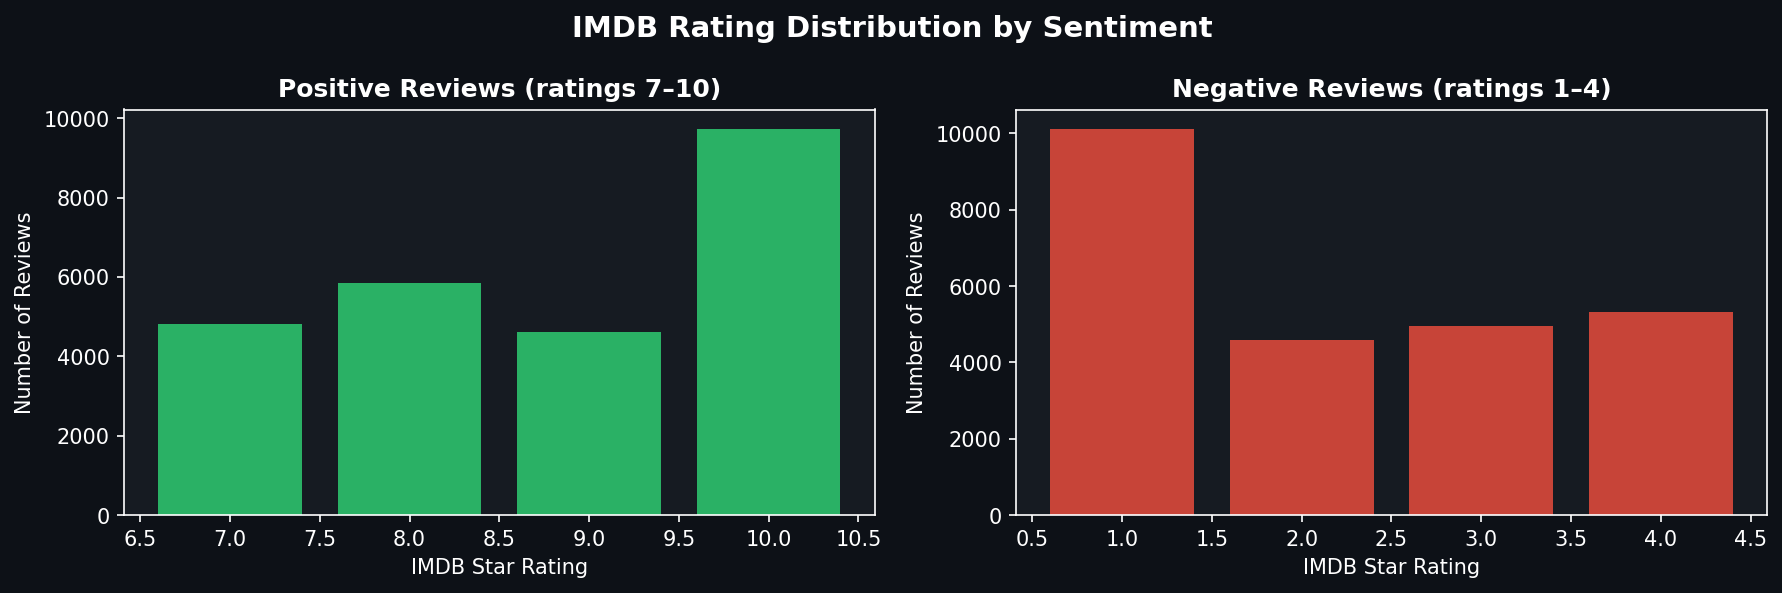
\includegraphics[width=1.0\linewidth]
      {../outputs/00_rating_distribution.png}\\[4pt]
    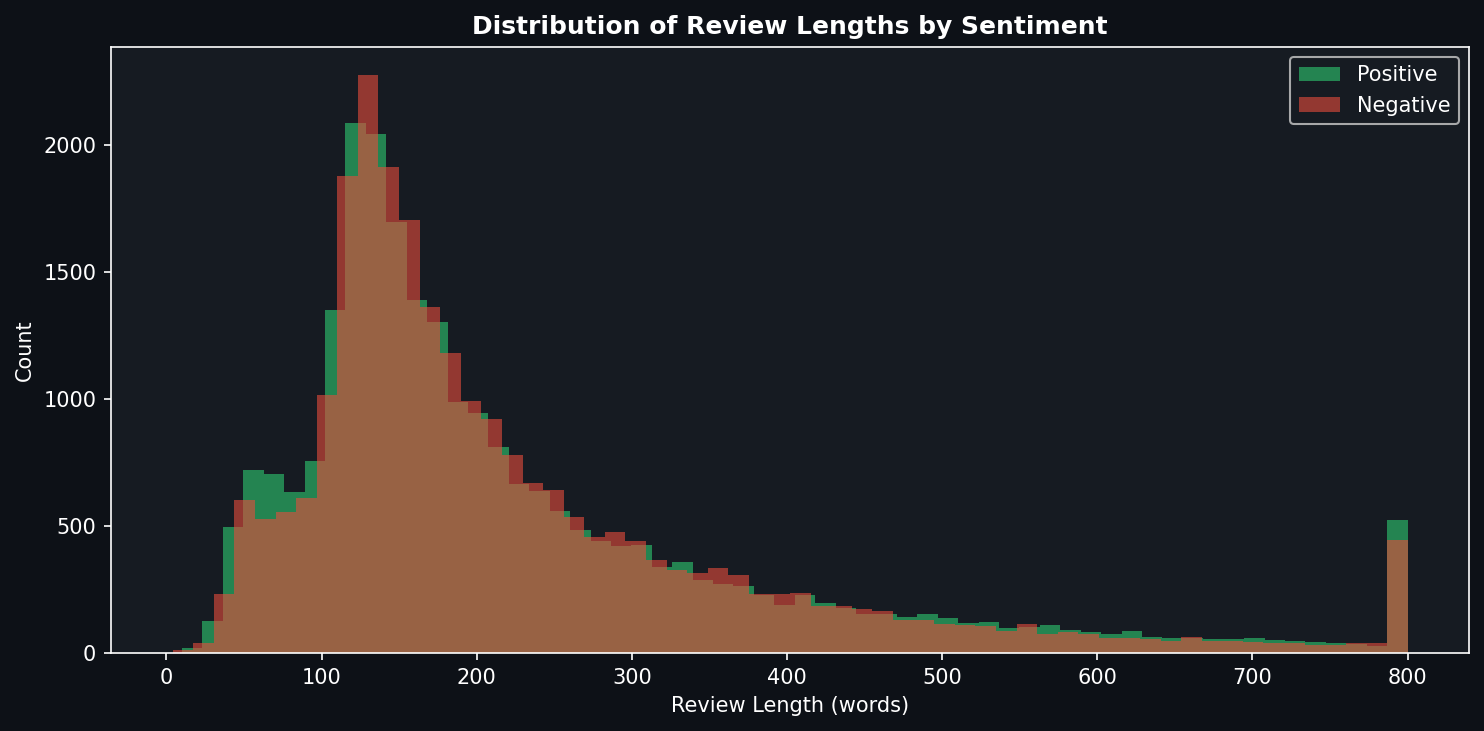
\includegraphics[width=0.85\linewidth]
      {../outputs/06_length_distribution.png}
  \end{center}
\end{columns}
\end{frame}

%% ─────────────────────────────────────────────────────────────────────────────
%% SLIDE 4 — PREPROCESSING
%% ─────────────────────────────────────────────────────────────────────────────
\begin{frame}[fragile]{NLP Preprocessing Pipeline}
\framesubtitle{7-step text cleaning before feature extraction}

\begin{columns}[T]
  \column{0.46\textwidth}
  \vspace{0.05cm}
  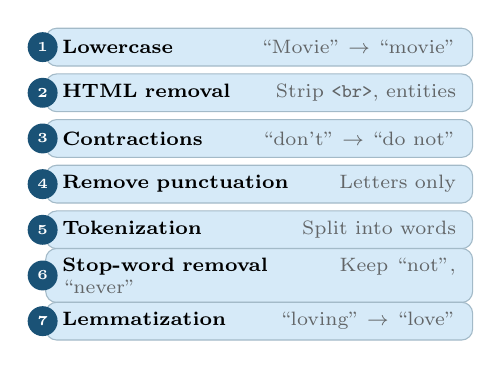
\begin{tikzpicture}[
    pbox/.style={
      draw=primary!40,fill=primarylt,rounded corners=4pt,
      minimum width=5.4cm,minimum height=0.48cm,
      align=left,text width=5.0cm,inner xsep=6pt,font=\scriptsize},
    num/.style={circle,fill=primary,text=white,
      font=\tiny\bfseries,minimum size=0.38cm,inner sep=0pt},
  ]
    \node[pbox] at (3,0.00)
      {\textbf{Lowercase}\hfill{\color{txtsub}``Movie'' $\to$ ``movie''}};
    \node[num] at (0.25,0.00){1};

    \node[pbox] at (3,-0.58)
      {\textbf{HTML removal}\hfill{\color{txtsub}Strip \texttt{<br>}, entities}};
    \node[num] at (0.25,-0.58){2};

    \node[pbox] at (3,-1.16)
      {\textbf{Contractions}\hfill{\color{txtsub}``don't'' $\to$ ``do not''}};
    \node[num] at (0.25,-1.16){3};

    \node[pbox] at (3,-1.74)
      {\textbf{Remove punctuation}\hfill{\color{txtsub}Letters only}};
    \node[num] at (0.25,-1.74){4};

    \node[pbox] at (3,-2.32)
      {\textbf{Tokenization}\hfill{\color{txtsub}Split into words}};
    \node[num] at (0.25,-2.32){5};

    \node[pbox] at (3,-2.90)
      {\textbf{Stop-word removal}\hfill{\color{txtsub}Keep ``not'', ``never''}};
    \node[num] at (0.25,-2.90){6};

    \node[pbox] at (3,-3.48)
      {\textbf{Lemmatization}\hfill{\color{txtsub}``loving'' $\to$ ``love''}};
    \node[num] at (0.25,-3.48){7};
  \end{tikzpicture}

  \vspace{0.15cm}
  \begin{tcolorbox}[enhanced,colback=panelbg,colframe=txtsub!30,
      arc=3pt,boxrule=0.5pt,top=3pt,bottom=3pt,left=5pt,right=5pt]
    \small
    \textbf{Before:}\ \texttt{<br>I DON'T think this is Good!!! WORST 2hrs}\\[2pt]
    \textbf{After:}\ \ \texttt{not think good worst hour}
  \end{tcolorbox}

  \column{0.50\textwidth}
  \begin{tcolorbox}[codebox]
  \begin{lstlisting}[style=py, numbers=none]
from bs4 import BeautifulSoup
from nltk.corpus import stopwords
from nltk.stem import WordNetLemmatizer

KEEP = {"not", "no", "never"}
stops = set(stopwords.words('english'))
stops -= KEEP
lem = WordNetLemmatizer()

def preprocess(text):
    text = BeautifulSoup(
        text, "html.parser").get_text()
    text = re.sub(r"[^a-z\s]", "",
                  text.lower())
    return " ".join([
        lem.lemmatize(w)
        for w in text.split()
        if w not in stops
    ])
  \end{lstlisting}
  \end{tcolorbox}

  \vspace{0.15cm}
  \begin{tcolorbox}[enhanced,colback=pgreenlt,colframe=pgreen,
      boxrule=0pt,leftrule=3pt,arc=2pt,
      top=3pt,bottom=3pt,left=6pt,right=6pt]
    \tiny\textbf{Key insight:} Negation words (``not'', ``never'') are
    preserved --- removing them would flip sentiment signals.
    ``\textit{not good}'' $\neq$ ``\textit{good}''.
  \end{tcolorbox}
\end{columns}
\end{frame}

%% ─────────────────────────────────────────────────────────────────────────────
%% SLIDE 5 — TF-IDF & TOP WORDS
%% ─────────────────────────────────────────────────────────────────────────────
\begin{frame}{TF-IDF Feature Extraction --- Top Predictive Words}
\framesubtitle{Logistic Regression coefficient weights reveal strongest sentiment signals}

\begin{columns}[T]
  \column{0.36\textwidth}
  \vspace{0.1cm}

  \begin{tcolorbox}[enhanced,colback=panelbg,colframe=primary!30,
      arc=3pt,boxrule=0.5pt,
      title={\small\bfseries\color{primary} TF-IDF Formula},
      coltitle=primary,
      top=4pt,bottom=4pt,left=5pt,right=5pt]
    \small
    \[
      \mathrm{score}(t,d) =
        \log(1+f_{t,d})
        \cdot
        \log\!\tfrac{N+1}{df_t+1}
    \]
    {\tiny\color{txtsub}
    $f_{t,d}$: term count in doc;
    $N$: corpus size; $df_t$: doc freq.}
  \end{tcolorbox}

  \vspace{0.25cm}
  {\scriptsize
  \rowcolors{2}{primarylt!60}{white}
  \begin{tabular}{@{}ll@{}}
    \toprule
    \rowcolor{primary!15}\textbf{Parameter} & \textbf{Value}\\
    \midrule
    \texttt{max\_features}  & 10,000 \\
    \texttt{ngram\_range}   & (1, 2) \\
    \texttt{min\_df}        & 2 \\
    \texttt{max\_df}        & 0.95 \\
    \texttt{sublinear\_tf}  & True \\
    Matrix shape            & 40K $\times$ 10K \\
    \bottomrule
  \end{tabular}
  }

  \begin{tcolorbox}[enhanced,colback=accentlt,colframe=accent,
      boxrule=0pt,leftrule=3pt,arc=2pt,
      top=3pt,bottom=3pt,left=5pt,right=5pt]
    \small Bigrams capture phrases like \textit{``must see''},
    \textit{``not disappoint''}, \textit{``waste of time''}.
  \end{tcolorbox}

  \column{0.61\textwidth}
  \begin{center}
    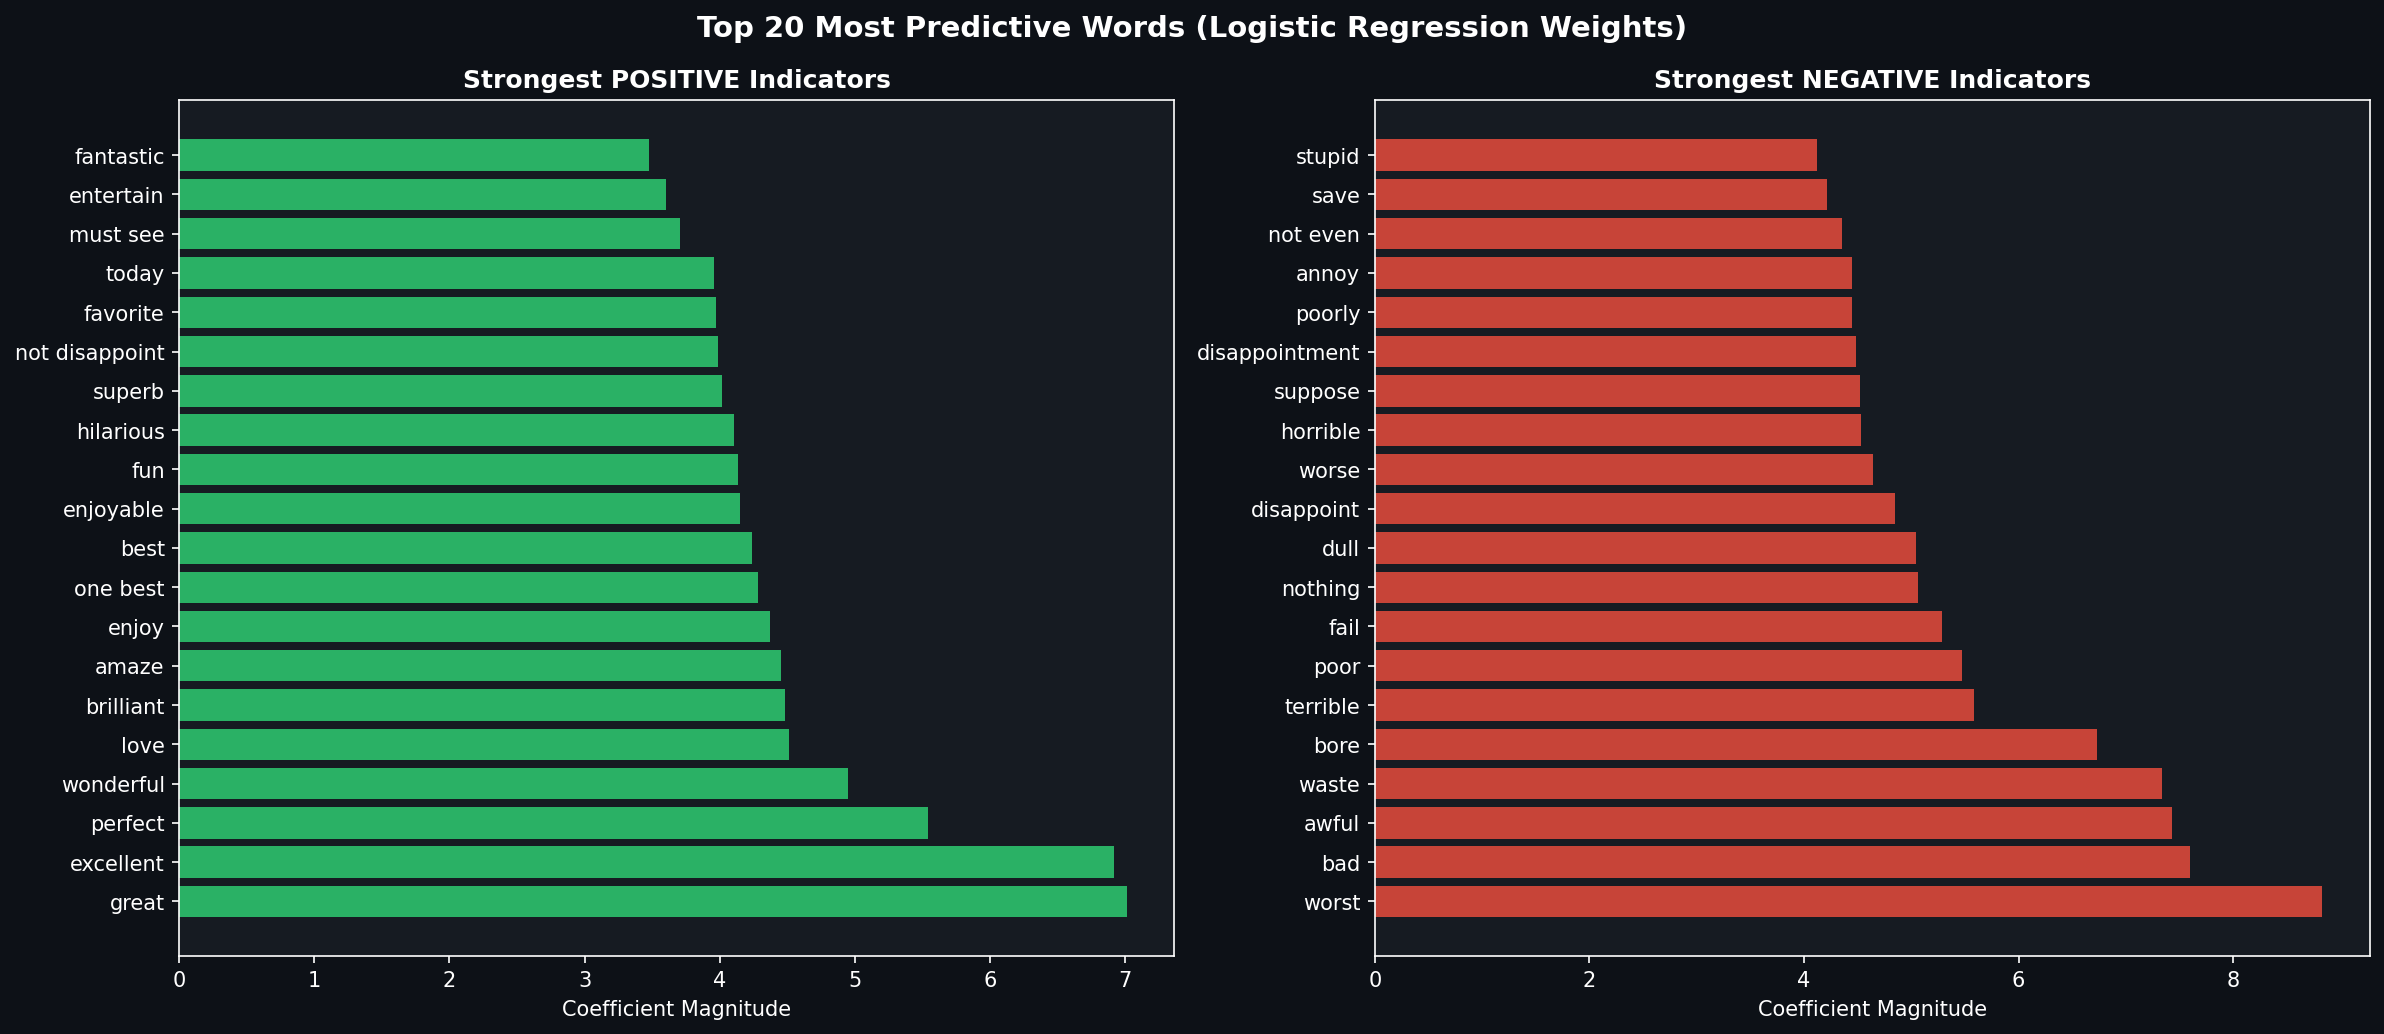
\includegraphics[width=1.06\linewidth]
      {../outputs/04_top_words.png}
  \end{center}
\end{columns}
\end{frame}

%% ─────────────────────────────────────────────────────────────────────────────
%% SLIDE 6 — MODEL COMPARISON
%% ─────────────────────────────────────────────────────────────────────────────
\begin{frame}{Model Comparison --- 5 Classifiers Benchmarked}
\framesubtitle{All models trained on identical TF-IDF features; LogReg + TF-IDF wins}

\begin{columns}[T]
  \column{0.62\textwidth}
  \begin{center}
    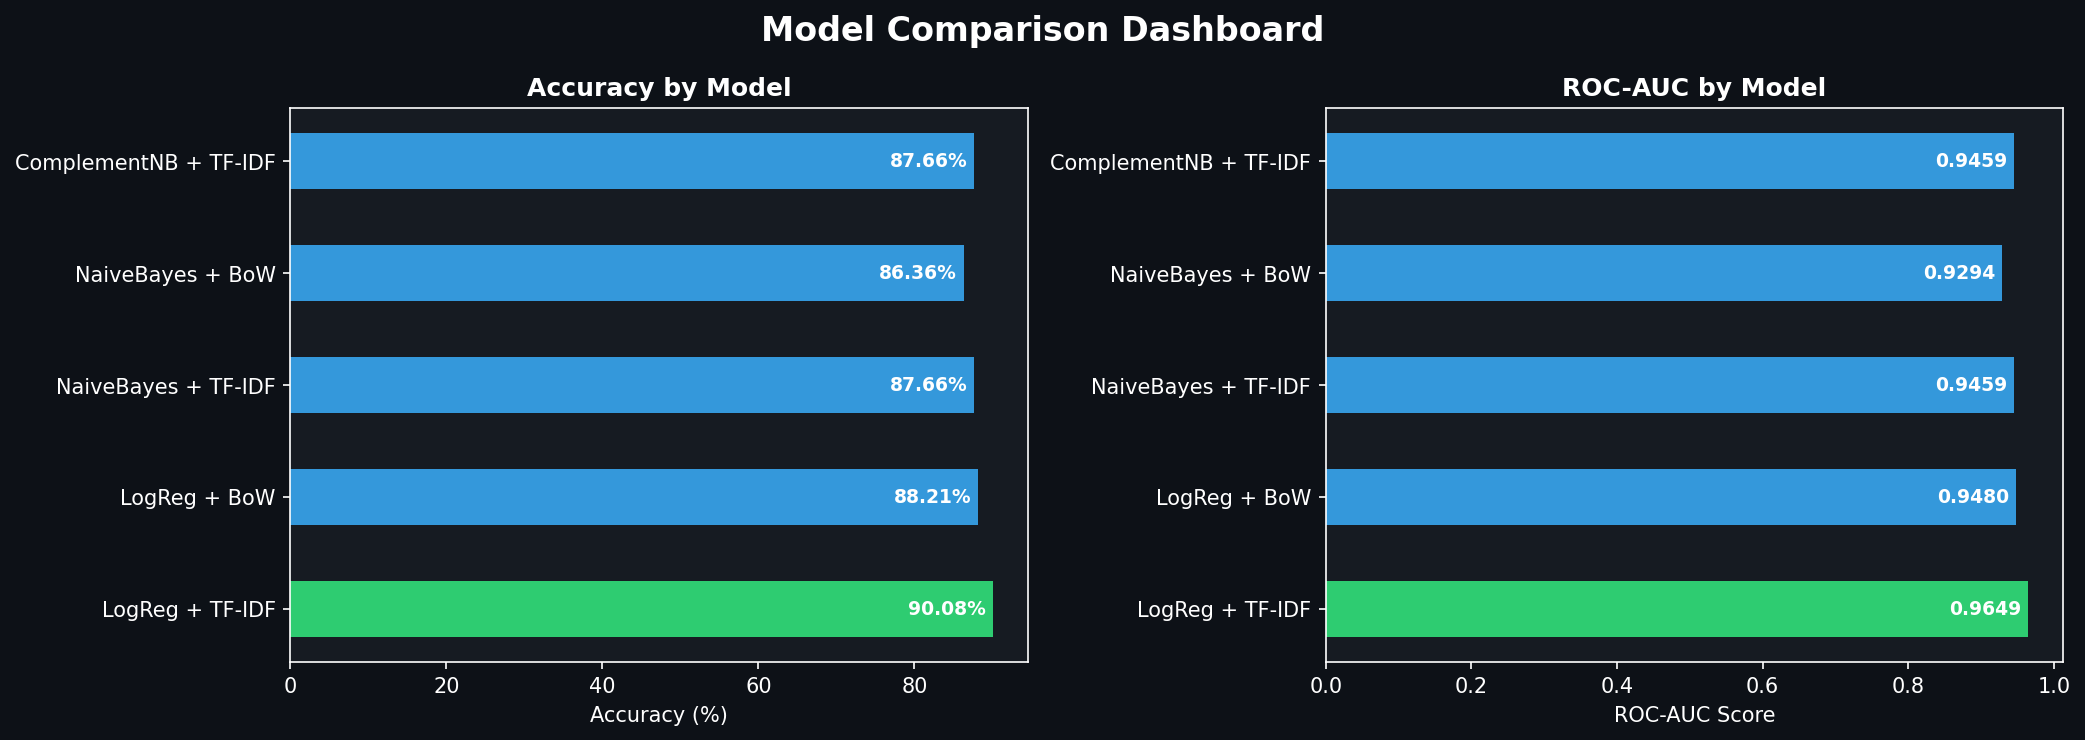
\includegraphics[width=\linewidth,height=5.4cm,keepaspectratio]
      {../outputs/01_model_comparison.png}
  \end{center}

  \column{0.35\textwidth}
  \vspace{0.2cm}

  \begin{tcolorbox}[enhanced,colback=accentlt,colframe=accent,
      arc=4pt,boxrule=1pt,
      title={\small\bfseries\color{accent} Best: LogReg + TF-IDF},
      coltitle=accent,
      top=4pt,bottom=4pt,left=6pt,right=6pt]
    \scriptsize
    \begin{tabular}{@{}ll@{}}
      \textbf{Accuracy}  & 90.08\% \\
      \textbf{ROC-AUC}   & 0.9649  \\
    \end{tabular}
  \end{tcolorbox}

  \vspace{0.2cm}
  {\scriptsize
  \rowcolors{2}{primarylt!60}{white}
  \begin{tabular}{@{}lc@{}}
    \toprule
    \rowcolor{primary!15}\textbf{Model} & \textbf{Acc.}\\
    \midrule
    NaiveBayes + BoW   & 86.36\% \\
    NaiveBayes + TF-IDF& 87.66\% \\
    ComplementNB + TFIDF & 87.66\% \\
    LogReg + BoW       & 88.21\% \\
    \textbf{LogReg + TF-IDF} & \textbf{90.08\%} \\
    \bottomrule
  \end{tabular}
  }

  \vspace{0.2cm}
  \begin{tcolorbox}[enhanced,colback=primarylt,colframe=primary,
      boxrule=0pt,leftrule=3pt,arc=2pt,
      top=3pt,bottom=3pt,left=5pt,right=5pt]
    \tiny TF-IDF consistently beats BoW by giving
    rare, informative words higher weight.
  \end{tcolorbox}
\end{columns}
\end{frame}

%% ─────────────────────────────────────────────────────────────────────────────
%% SLIDE 7 — SKLEARN PIPELINE CODE
%% ─────────────────────────────────────────────────────────────────────────────
%% ─── SLIDE 1 of 2: Pipeline Definition + Architecture ───────────────────────
\begin{frame}[fragile]{Scikit-learn Pipeline --- Code (1/2)}
\framesubtitle{TF-IDF + Logistic Regression chained in a single Pipeline object}

\begin{columns}[T]
  %% ── Left: build code ──────────────────────────────────────────────────────
  \column{0.50\textwidth}
  \vspace{-0.4cm}
  \begin{tcolorbox}[codebox]
  \begin{lstlisting}[style=py, numbers=none]
from sklearn.pipeline import Pipeline
from sklearn.linear_model import \
    LogisticRegression
from sklearn.feature_extraction.text \
    import TfidfVectorizer
import joblib
# Build pipeline
pipeline = Pipeline([
  ('tfidf', TfidfVectorizer(
      max_features=10_000,
      ngram_range=(1, 2),
      sublinear_tf=True,
      min_df=2,max_df=0.95,
  )),('clf', LogisticRegression(
      C=1.0,
      max_iter=1000,
      solver='lbfgs',)),])
# Train & evaluate
pipeline.fit(X_train, y_train)
acc = pipeline.score(X_test, y_test)
print(f"Accuracy: {acc:.4f}") 
# Save trained model for API
joblib.dump(pipeline, 'sentiment_model.pkl')
  \end{lstlisting}
  \end{tcolorbox}

  %% ── Right: architecture diagram ───────────────────────────────────────────
  \column{0.46\textwidth}
  \vspace{0.3cm}
  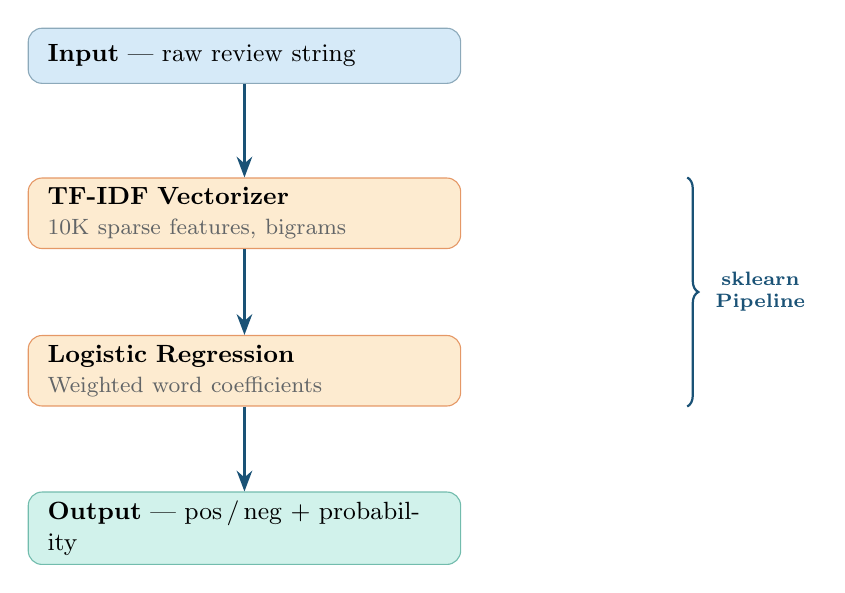
\begin{tikzpicture}[
    bx/.style={draw=primary!50,fill=primarylt,rounded corners=5pt,
      minimum width=5.4cm,minimum height=0.70cm,
      align=left,text width=5.0cm,inner xsep=7pt,font=\small},
    hx/.style={draw=accent!60,fill=accentlt,rounded corners=5pt,
      minimum width=5.4cm,minimum height=0.70cm,
      align=left,text width=5.0cm,inner xsep=7pt,font=\small},
    gx/.style={draw=teal!60,fill=teallt,rounded corners=5pt,
      minimum width=5.4cm,minimum height=0.70cm,
      align=left,text width=5.0cm,inner xsep=7pt,font=\small},
    ar/.style={-{Stealth},primary,line width=1pt},
  ]
    \node[bx] (i) at (0,0)
      {\textbf{Input} --- raw review string};
    \node[hx] (t) at (0,-2.0)
      {\textbf{TF-IDF Vectorizer}\\
       {\footnotesize\color{txtsub}10K sparse features, bigrams}};
    \node[hx] (c) at (0,-4.0)
      {\textbf{Logistic Regression}\\
       {\footnotesize\color{txtsub}Weighted word coefficients}};
    \node[gx] (o) at (0,-6.0)
      {\textbf{Output} --- pos\,/\,neg + probability};

    \draw[ar](i)--(t); \draw[ar](t)--(c); \draw[ar](c)--(o);

    \draw[decorate,decoration={brace,amplitude=4pt,raise=2pt},
      primary,thick]
      ([xshift=2.8cm]t.north east)--([xshift=2.8cm]c.south east)
      node[midway,xshift=1.0cm,font=\scriptsize\bfseries,color=primary,
           align=center,text width=1.2cm]{sklearn\\Pipeline};
  \end{tikzpicture}
\end{columns}
\end{frame}


%% ─── SLIDE 2 of 2: Why Pipeline? + API Usage ────────────────────────────────
\begin{frame}[fragile]{Scikit-learn Pipeline --- Usage (2/2)}
\framesubtitle{Deployment \& cross-validation benefits}

\begin{columns}[T]
  %% ── Left: Why Pipeline? ───────────────────────────────────────────────────
  \column{0.48\textwidth}
  \vspace{-0.2cm}

  \begin{tcolorbox}[enhanced,colback=pgreenlt,colframe=pgreen,
      boxrule=0pt,leftrule=4pt,arc=3pt,
      top=8pt,bottom=8pt,left=8pt,right=8pt]
    \small\textbf{Why Pipeline?}

    \vspace{4pt}
    \small Wrapping the vectorizer and model in a single
    \texttt{Pipeline} object provides two key guarantees:

    \vspace{6pt}
    \begin{itemize}\setlength\itemsep{4pt}
      \item \textbf{No data leakage} --- the vectorizer is
            fit only on training folds during cross-validation,
            never on held-out data.
      \item \textbf{Trivial deployment} --- the entire
            fitted pipeline is serialised in one
            \texttt{joblib.dump()} call and loaded as a
            single object at inference time.
    \end{itemize}
  \end{tcolorbox}

  %% ── Right: Load & predict ─────────────────────────────────────────────────
  \column{0.48\textwidth}
  \vspace{-0.2cm}

  \begin{tcolorbox}[codebox]
  \begin{lstlisting}[style=py, numbers=none]
# Load & predict (in API)
model = joblib.load('sentiment_model.pkl')

pred = model.predict(
    ["Great film!"]
)
# -> ['pos']

prob = model.predict_proba(
    ["Great film!"]
)
# -> [[0.08, 0.92]]
  \end{lstlisting}
  \end{tcolorbox}

  \vspace{0.3cm}
  \begin{tcolorbox}[enhanced,colback=primarylt,colframe=primary!50,
      boxrule=0pt,leftrule=4pt,arc=3pt,
      top=6pt,bottom=6pt,left=8pt,right=8pt]
    \small\textbf{One object, full chain:}
    \texttt{model.predict()} runs TF-IDF
    vectorisation \emph{then} classification
    automatically --- no manual pre-processing
    step at inference time.
  \end{tcolorbox}

\end{columns}
\end{frame}

%% ─────────────────────────────────────────────────────────────────────────────
%% SLIDE 8 — EVALUATION
%% ─────────────────────────────────────────────────────────────────────────────
\begin{frame}{Model Evaluation \& Performance}
\framesubtitle{LogReg + TF-IDF evaluated on the held-out 10,000-review test set}

\begin{columns}[T]
  \column{0.38\textwidth}
  \begin{center}
    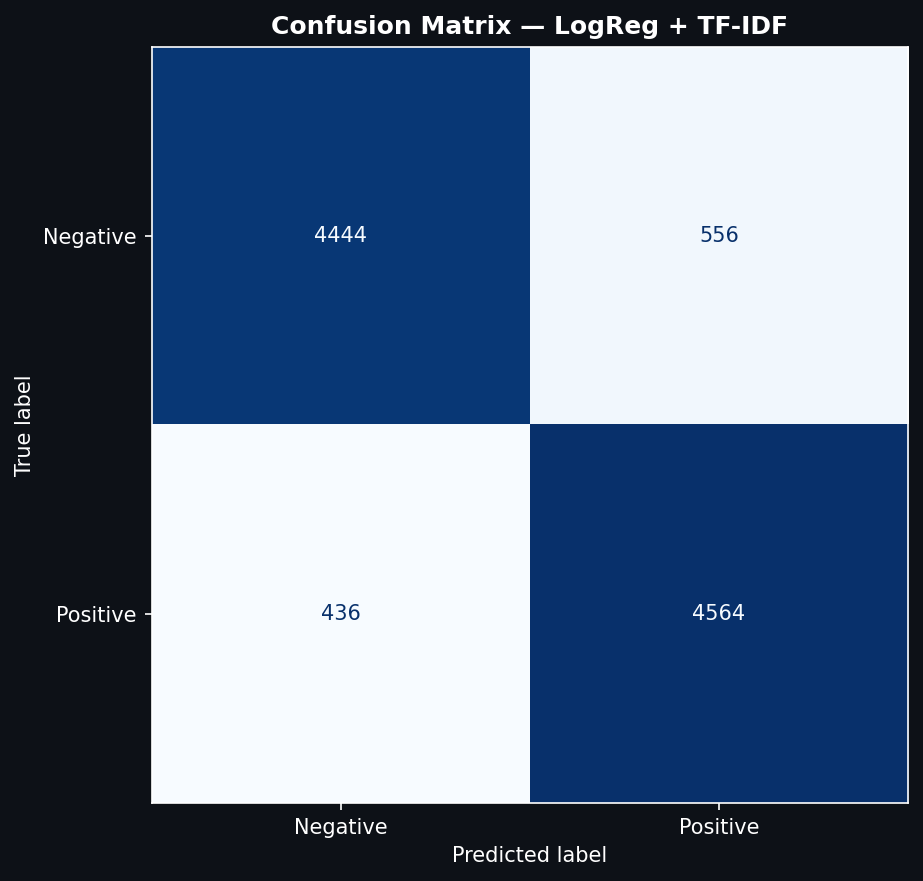
\includegraphics[width=\linewidth,height=4.0cm,keepaspectratio]
      {../outputs/02_confusion_matrix.png}
  \end{center}

  \vspace{0.1cm}
  {\scriptsize
  \rowcolors{2}{primarylt!60}{white}
  \begin{tabular}{@{}lcccc@{}}
    \toprule
    \rowcolor{primary!15}\textbf{Class} & \textbf{Prec} & \textbf{Rec} & \textbf{F1} & \textbf{N}\\
    \midrule
    Negative & 0.889 & 0.888 & 0.889 & 5000\\
    Positive & 0.913 & 0.913 & 0.913 & 5000\\
    \textbf{Avg}  & \textbf{0.901} & \textbf{0.901} & \textbf{0.901} & 10K\\
    \bottomrule
  \end{tabular}
  }

  \column{0.59\textwidth}
  \begin{center}
    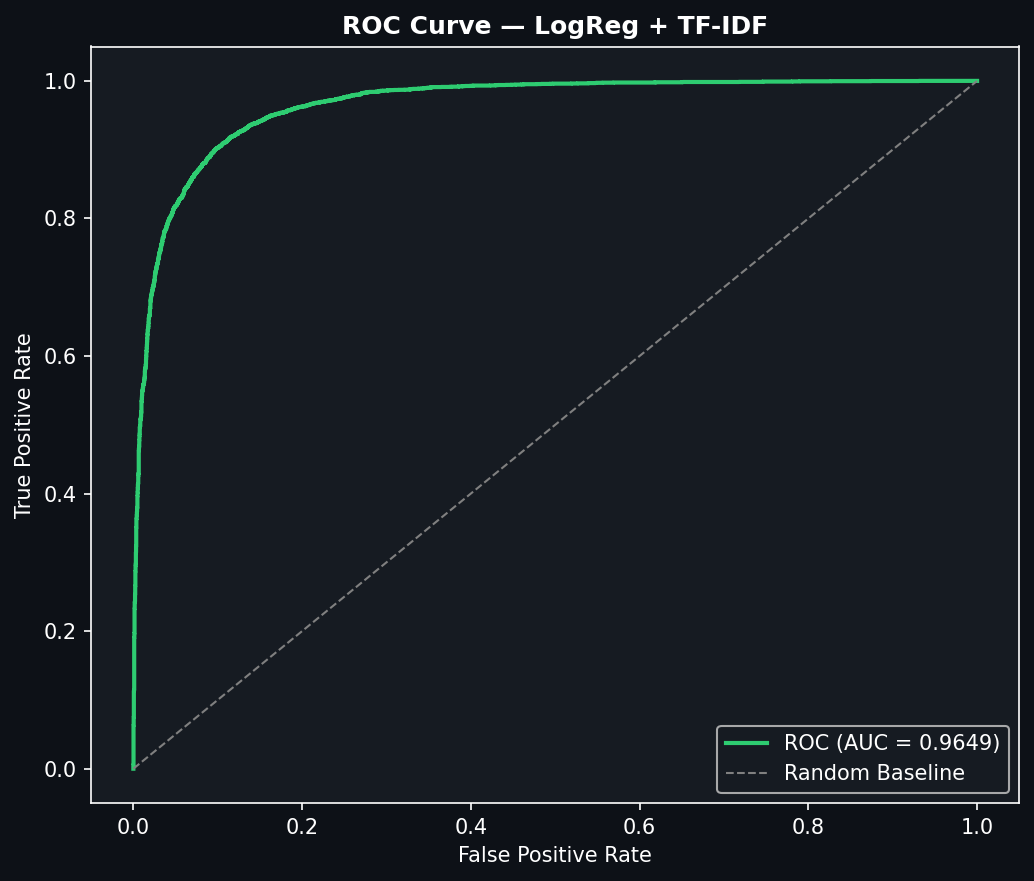
\includegraphics[width=\linewidth,height=5.4cm,keepaspectratio]
      {../outputs/03_roc_curve.png}
  \end{center}
\end{columns}
\end{frame}

%% ─────────────────────────────────────────────────────────────────────────────
%% SLIDE 9 — WORD CLOUDS
%% ─────────────────────────────────────────────────────────────────────────────
\begin{frame}{Exploratory Data Analysis --- Word Clouds}
\framesubtitle{Most frequent words in positive vs.\ negative reviews after preprocessing}

\begin{center}
  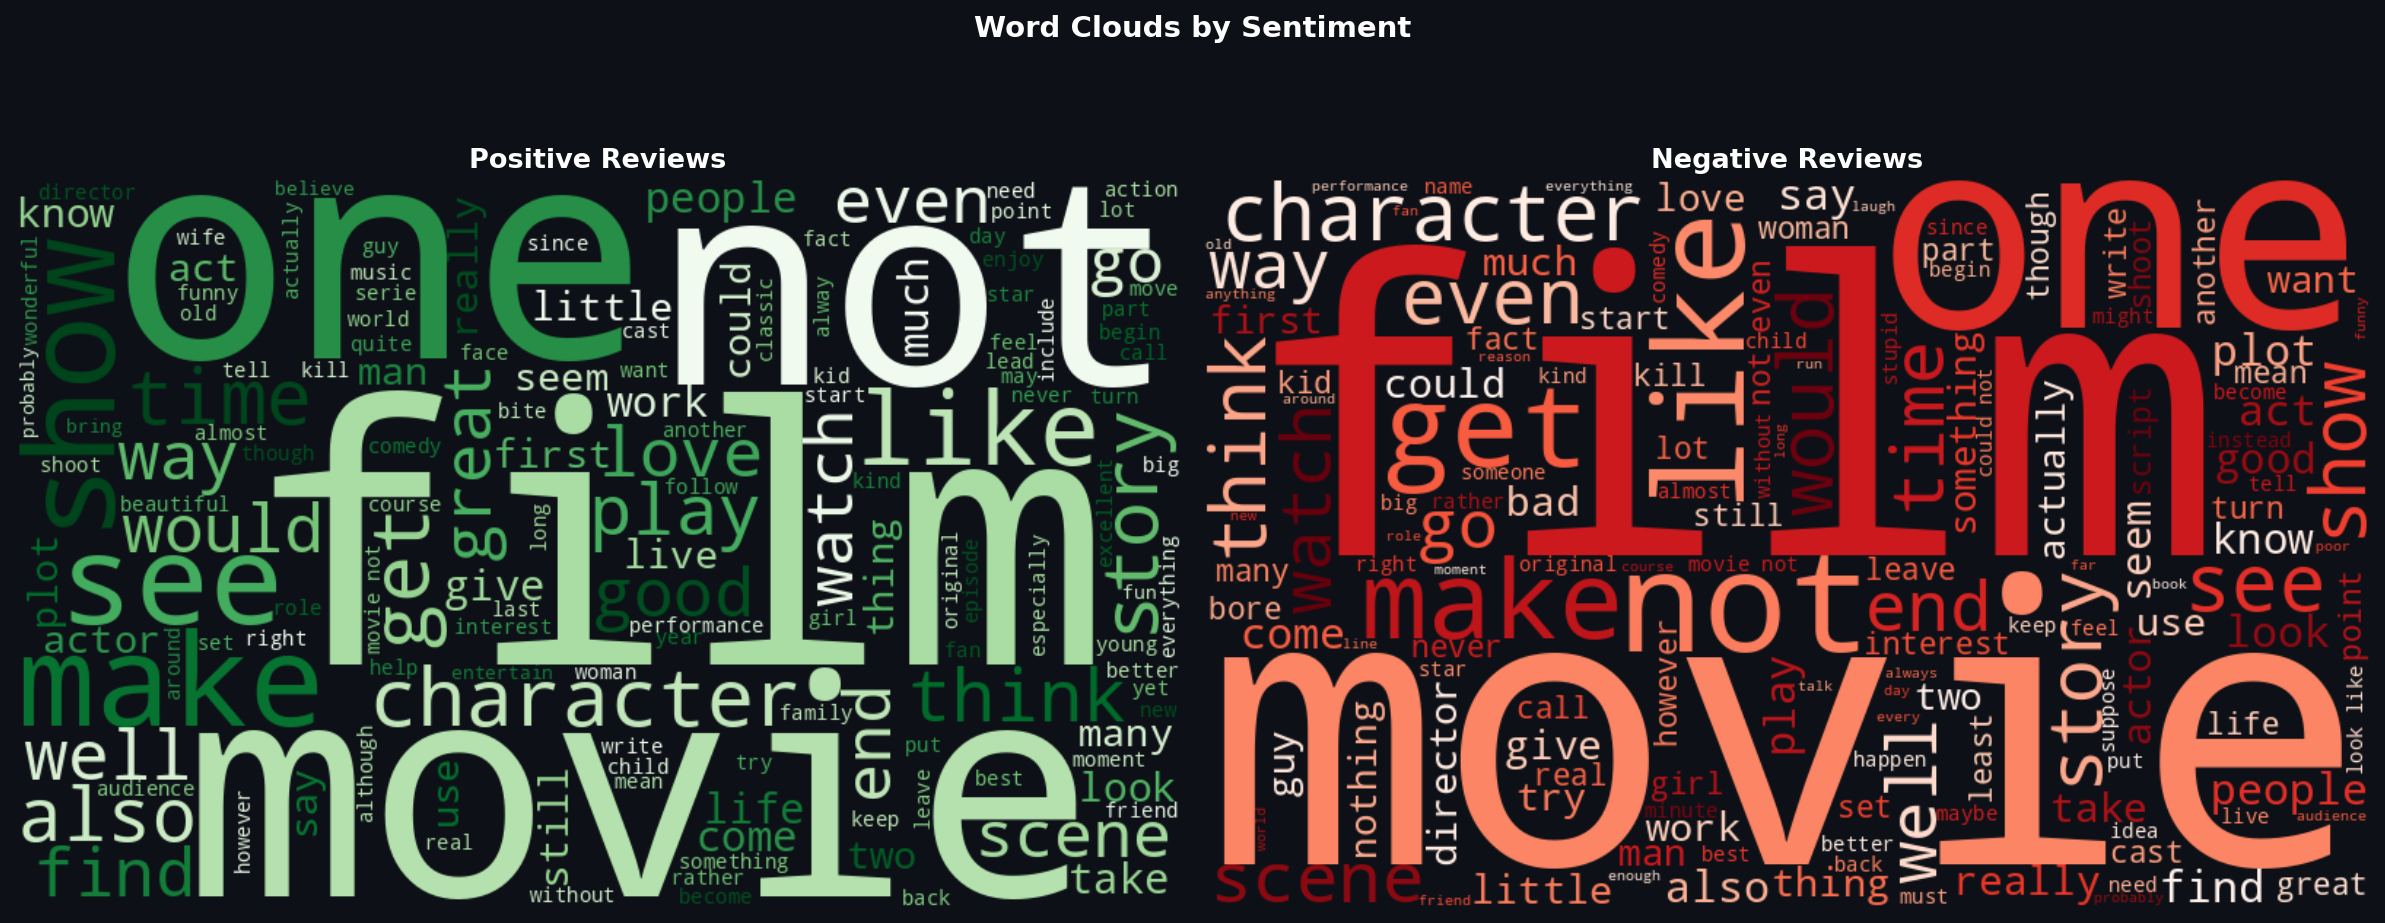
\includegraphics[width=0.96\linewidth,height=5.5cm,keepaspectratio]
    {../outputs/05_wordclouds.png}
\end{center}

\vspace{0.1cm}
\begin{columns}[T]
  \column{0.48\textwidth}
  \begin{tcolorbox}[enhanced,colback=pgreenlt,colframe=pgreen,
      boxrule=0pt,leftrule=3pt,arc=2pt,
      top=3pt,bottom=3pt,left=6pt,right=6pt]
    \scriptsize\textbf{Positive cloud:} Words like \textit{great},
    \textit{love}, \textit{brilliant}, \textit{enjoy}, \textit{perfect}
    dominate --- strong praise vocabulary.
  \end{tcolorbox}

  \column{0.48\textwidth}
  \begin{tcolorbox}[enhanced,colback=predlt,colframe=pred,
      boxrule=0pt,leftrule=3pt,arc=2pt,
      top=3pt,bottom=3pt,left=6pt,right=6pt]
    \scriptsize\textbf{Negative cloud:} Words like \textit{bad},
    \textit{worst}, \textit{waste}, \textit{bore}, \textit{terrible}
    stand out --- clear disappointment signals.
  \end{tcolorbox}
\end{columns}
\end{frame}

%% ─────────────────────────────────────────────────────────────────────────────
%% SLIDE 10 — FASTAPI BACKEND
%% ─────────────────────────────────────────────────────────────────────────────
\begin{frame}[fragile]{FastAPI Backend --- sentiment\_api.py}
\framesubtitle{Production-ready REST server with Pydantic validation and CORS}

\begin{columns}[T]
  \column{0.46\textwidth}
  % Request flow
  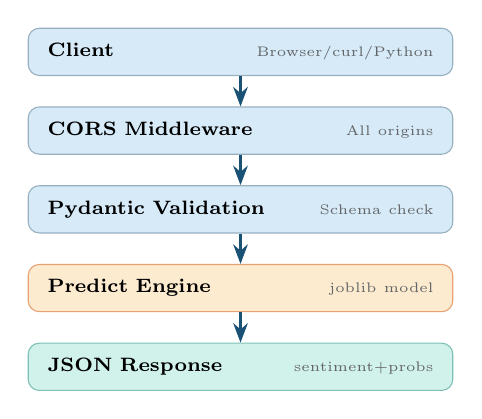
\begin{tikzpicture}[
    ly/.style={draw=primary!45,fill=primarylt,rounded corners=4pt,
      minimum width=5.3cm,minimum height=0.60cm,
      align=left,text width=4.9cm,inner xsep=7pt,font=\scriptsize},
    la/.style={draw=accent!55,fill=accentlt,rounded corners=4pt,
      minimum width=5.3cm,minimum height=0.60cm,
      align=left,text width=4.9cm,inner xsep=7pt,font=\scriptsize},
    lg/.style={draw=teal!55,fill=teallt,rounded corners=4pt,
      minimum width=5.3cm,minimum height=0.60cm,
      align=left,text width=4.9cm,inner xsep=7pt,font=\scriptsize},
    ar/.style={-{Stealth},primary,line width=0.9pt},
  ]
    \node[ly](r) at (0,0)
      {\textbf{Client}\hfill{\tiny\color{txtsub}Browser/curl/Python}};
    \node[ly](m) at (0,-1.0)
      {\textbf{CORS Middleware}\hfill{\tiny\color{txtsub}All origins}};
    \node[ly](v) at (0,-2.0)
      {\textbf{Pydantic Validation}\hfill{\tiny\color{txtsub}Schema check}};
    \node[la](p) at (0,-3.0)
      {\textbf{Predict Engine}\hfill{\tiny\color{txtsub}joblib model}};
    \node[lg](o) at (0,-4.0)
      {\textbf{JSON Response}\hfill{\tiny\color{txtsub}sentiment+probs}};
    \draw[ar](r)--(m);\draw[ar](m)--(v);
    \draw[ar](v)--(p);\draw[ar](p)--(o);
  \end{tikzpicture}

  \vspace{0.2cm}
  {\scriptsize
  \rowcolors{2}{primarylt!60}{white}
  \begin{tabular}{@{}lll@{}}
    \toprule
    \rowcolor{primary!15}\textbf{Method} & \textbf{Route} & \textbf{Use}\\
    \midrule
    \textcolor{pgreen}{\textbf{GET}} & \texttt{/} & HTML UI\\
    \textcolor{pgreen}{\textbf{GET}} & \texttt{/health} & Status\\
    \textcolor{accent}{\textbf{POST}}& \texttt{/predict} & Single\\
    \textcolor{accent}{\textbf{POST}}& \texttt{/batch\_predict} & Batch\\
    \textcolor{pgreen}{\textbf{GET}} & \texttt{/docs} & Swagger\\
    \bottomrule
  \end{tabular}
  }

  \column{0.50\textwidth}
  \vspace{-0.4cm}
  \begin{tcolorbox}[codebox]
  \begin{lstlisting}[style=json, numbers=none]
// POST /predict  -- Request
{ "text": "This movie is fantastic!" }
// Response (200 OK)
{ "text":         "This movie ...",
  "sentiment":    "positive","confidence":   0.9453,
  "positive_prob":0.9453,"negative_prob":0.0547,
  "timestamp":    "2026-03-03T..."}
  \end{lstlisting}
  \end{tcolorbox}

  \vspace{-0.15cm}
  \begin{tcolorbox}[codebox]
  \begin{lstlisting}[style=json, numbers=none]
// POST /batch_predict
{ "texts": ["Great!", "Terrible."] }
// Response
{ "predictions": [{...}, {...}],
  "total": 2,"processing_time_ms": 8.3 }
  \end{lstlisting}
  \end{tcolorbox}

  \vspace{-0.5cm}
  \begin{tcolorbox}[codebox]
  \begin{lstlisting}[style=py, numbers=none]
# Run server
uvicorn sentiment_api:app \
    --reload --port 8000
# Docs: localhost:8000/docs
  \end{lstlisting}
  \end{tcolorbox}
\end{columns}
\end{frame}

%% ─────────────────────────────────────────────────────────────────────────────
%% SLIDE 11 — WEB FRONTEND DEMO
%% ─────────────────────────────────────────────────────────────────────────────
\begin{frame}{Web Frontend Demo --- Live API Results}
\framesubtitle{HTML/CSS/JS frontend calling FastAPI --- actual screenshots}

\begin{columns}[c]
  \column{0.32\textwidth}
  \vspace{-2.5cm}
  \begin{center}
    {\scriptsize\bfseries\color{txtsub} Default State}\\[4pt]
    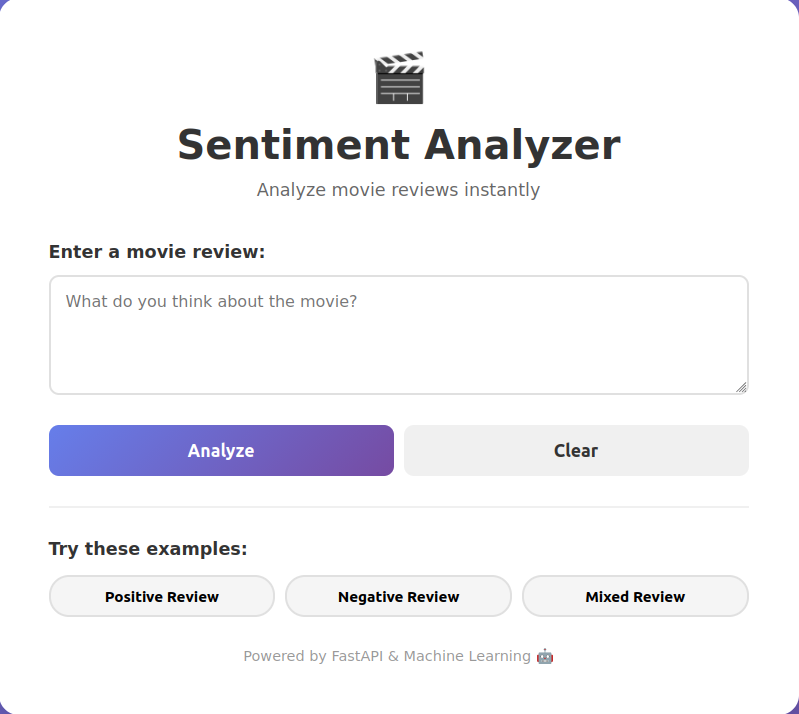
\includegraphics[width=\linewidth,keepaspectratio]
      {../outputs/sentiment_api.png}
  \end{center}

  \column{0.32\textwidth}
  \vspace{-0.5cm}
  \begin{center}
    {\scriptsize\bfseries\color{pgreen} Positive Result}\\[4pt]
    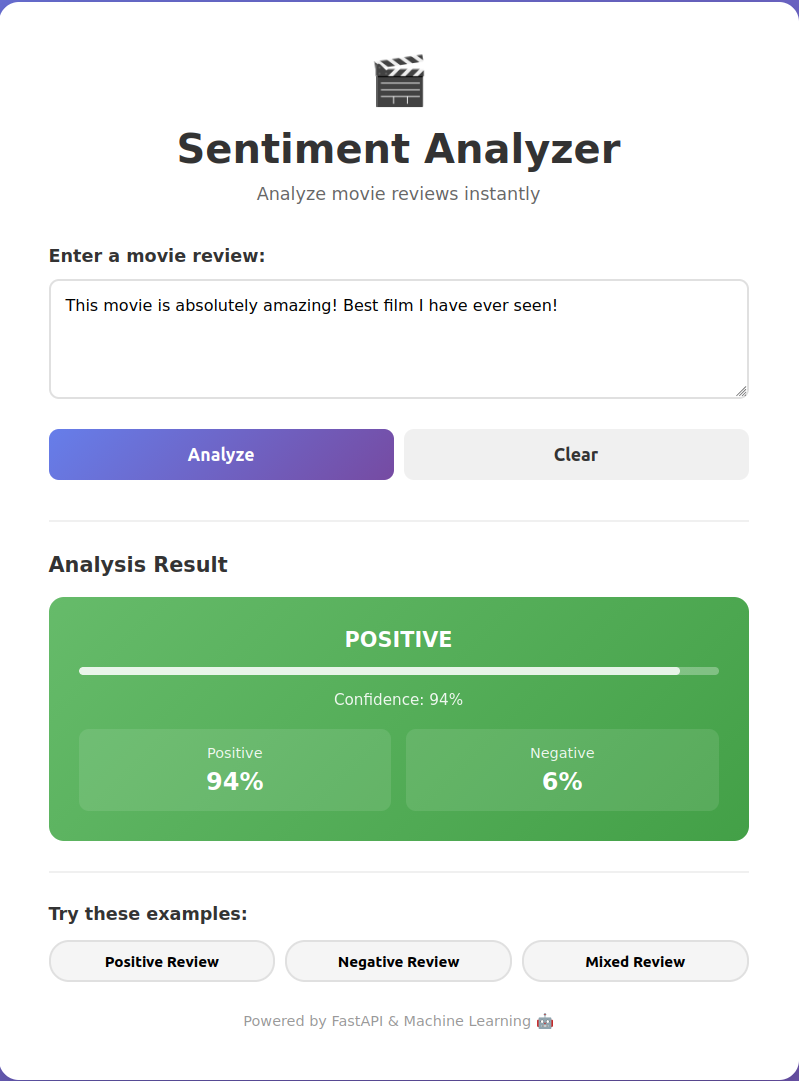
\includegraphics[width=\linewidth,keepaspectratio]
      {../outputs/pos_sentiment_api.png}
  \end{center}

  \column{0.32\textwidth}
  \vspace{-0.5cm}
  \begin{center}
    {\scriptsize\bfseries\color{pred} Negative Result}\\[4pt]
    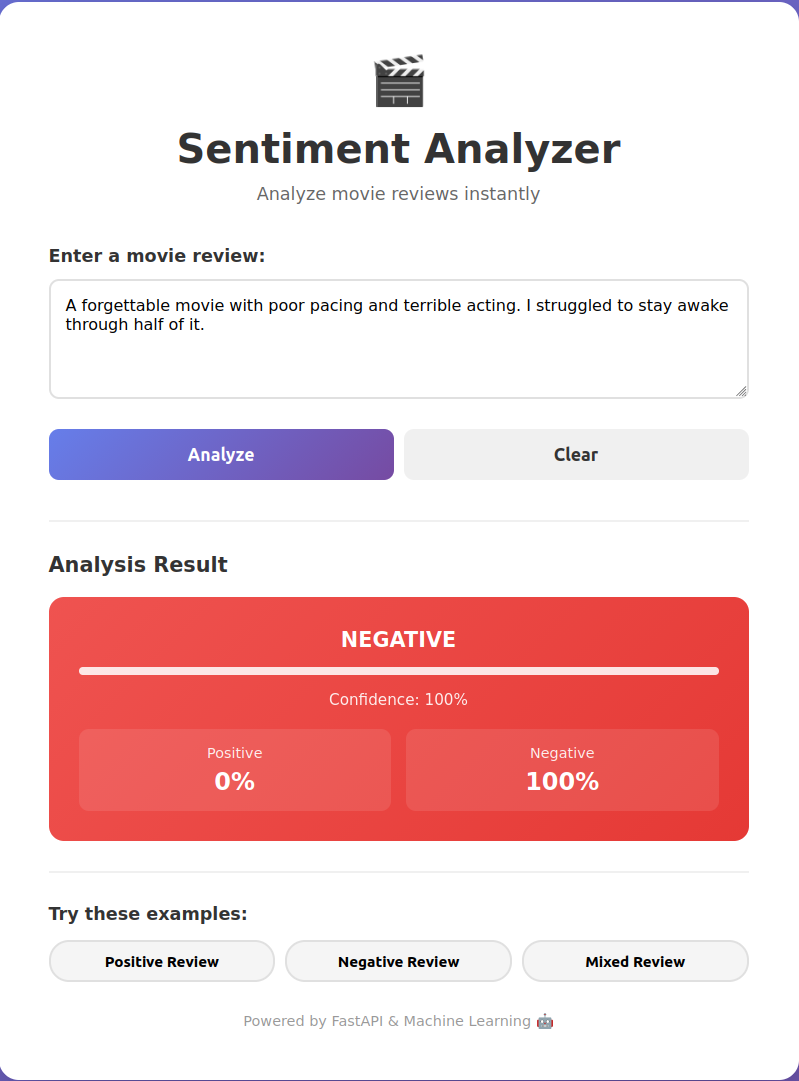
\includegraphics[width=\linewidth,keepaspectratio]
      {../outputs/neg_sentiment_api.png}
  \end{center}
\end{columns}

\vspace{-0.15cm}
\begin{columns}[T]
  \column{0.48\textwidth}
  \begin{tcolorbox}[enhanced,colback=pgreenlt,colframe=pgreen,
      boxrule=0pt,leftrule=3pt,arc=2pt,
      top=3pt,bottom=3pt,left=6pt,right=6pt]
    \scriptsize\textbf{Positive example:} ``This movie is absolutely amazing!
    Best film I have ever seen!'' $\to$ \textbf{94\% confidence}
  \end{tcolorbox}

  \column{0.48\textwidth}
  \begin{tcolorbox}[enhanced,colback=predlt,colframe=pred,
      boxrule=0pt,leftrule=3pt,arc=2pt,
      top=3pt,bottom=3pt,left=6pt,right=6pt]
    \scriptsize\textbf{Negative example:} ``A forgettable movie with poor
    pacing and terrible acting.'' $\to$ \textbf{100\% confidence}
  \end{tcolorbox}
\end{columns}
\end{frame}

%% ─────────────────────────────────────────────────────────────────────────────
%% SLIDE 12 — SUMMARY
%% ─────────────────────────────────────────────────────────────────────────────
{
\setbeamercolor{background canvas}{bg=primary}
\begin{frame}[plain]

\begin{tikzpicture}[remember picture,overlay]
  \fill[white,opacity=0.04]
    (current page.south west) circle(7cm);
  \fill[accent,opacity=0.10]
    (current page.north east)++(-2cm,-2cm) circle(4cm);
\end{tikzpicture}

\vspace{0.2cm}
\begin{center}
  {\color{primarylt}\scriptsize\texttt{SUMMARY}}\\[5pt]
  {\color{white}\Large\bfseries What Was Built \& What Comes Next}\\[5pt]
  \textcolor{accent}{\rule{9cm}{1.5pt}}
\end{center}

\vspace{0.2cm}
\begin{columns}[T]
  \column{0.48\textwidth}
  \begin{tcolorbox}[enhanced,
      colback=white!8!primary,colframe=white!30,
      arc=5pt,boxrule=0.6pt,
      title={\small\bfseries Project Deliverables},
      coltitle=white,
      top=4pt,bottom=4pt,left=6pt,right=6pt]
    \color{primarylt}\scriptsize
    \begin{itemize}\setlength\itemsep{2pt}
      \item[\textcolor{accent}{$\checkmark$}]
        50K IMDB reviews with 7-step NLP pipeline
      \item[\textcolor{accent}{$\checkmark$}]
        TF-IDF (10K features, bigrams)
      \item[\textcolor{accent}{$\checkmark$}]
        5 classifiers; LogReg+TF-IDF best at \textbf{90.08\%}
      \item[\textcolor{accent}{$\checkmark$}]
        ROC-AUC = 0.9649
      \item[\textcolor{accent}{$\checkmark$}]
        FastAPI: \texttt{/predict}, \texttt{/batch\_predict}
      \item[\textcolor{accent}{$\checkmark$}]
        Pydantic validation, CORS, Swagger docs
      \item[\textcolor{accent}{$\checkmark$}]
        Responsive HTML/JS frontend (live screenshots)
    \end{itemize}
  \end{tcolorbox}

  \column{0.48\textwidth}
  \begin{tcolorbox}[enhanced,
      colback=white!8!primary,colframe=accent!60,
      arc=5pt,boxrule=0.6pt,
      title={\small\bfseries Future Improvements},
      coltitle=accent!80,
      top=4pt,bottom=4pt,left=6pt,right=6pt]
    \color{primarylt}\scriptsize
    \begin{itemize}\setlength\itemsep{2pt}
      \item[\textcolor{white}{$\to$}] Fine-tune \textbf{BERT} for +5\% accuracy
      \item[\textcolor{white}{$\to$}] Multilingual (mBERT / XLM-R)
      \item[\textcolor{white}{$\to$}] Redis caching for repeated queries
      \item[\textcolor{white}{$\to$}] Docker + Kubernetes deployment
      \item[\textcolor{white}{$\to$}] CI/CD with GitHub Actions
      \item[\textcolor{white}{$\to$}] Aspect-based sentiment analysis
      \item[\textcolor{white}{$\to$}] Model drift monitoring
    \end{itemize}
  \end{tcolorbox}
\end{columns}

\vspace{0.25cm}
\begin{center}
  
\begin{tikzpicture}
    \node[fill=accent,rounded corners=4pt,text=white,
          font=\small\bfseries,inner sep=7pt]{%
      50K Reviews $\cdot$ TF-IDF $\cdot$ LogReg $\cdot$
      90.08\% Acc $\cdot$ FastAPI $\cdot$ Live Frontend};
  \end{tikzpicture}
\end{center}
\end{frame}
}

\end{document}